%
%===============>>  ГРУППА 11-6 МОДУЛЬ 8  <<=============
%
\setmodule{Вспомнить всё}

%BEGIN_FOLD % ====>>_____ Занятие 1 _____<<====
\begin{class}[number=1]
	\begin{listofex}
		\item Вычислить:
		\begin{enumcols}[itemcolumns=2]
			\item \( \sin150\degree\sin(-120\degree)\ctg(-225\degree) \)
			\item \( \tg\left( -\dfrac{17\pi}{4} \right)\sin\dfrac{14\pi}{3} \cos\left( -\dfrac{25\pi}{4}\right)\ \)
		\end{enumcols}
		\item Вычислите:
		\begin{tasks}(2)
			\task \(\dfrac{4 \cdot \sin61\degree}{\cos29\degree}\)
			\task \(\dfrac{2 \cdot \sin136\degree}{\sin68\degree \cdot \sin22\degree}\)
		\end{tasks}
		\item Вычислить:
		\begin{enumcols}[itemcolumns=1]
			\item \exercise{1117}
			\item \exercise{1119}
		\end{enumcols}
		\item Решить уравнение:
		\begin{tasks}(2)
			\task \( \sin x = \dfrac{1}{2} \)
			\task \( 2\sin x = -\sqrt{2} \)
			\task \( 3\tg x = \sqrt{3} \)
			\task \( \sin^2 x = \dfrac{1}{2} \)
		\end{tasks}
%		\item Решить неравенство:
%		\begin{tasks}(2)
%			\task \( \sin x > \dfrac{1}{2} \)
%			\task \( \cos x \le \dfrac{\sqrt{2}}{2} \)
%			\task \( \sin x < 1 \)
%			\task \( \sin x \ge -\dfrac{3}{2}\)
%		\end{tasks}
		\item  Решите уравнение \( 8\sin x + 4\cos^2 x = 7 \)
		\item  Решите уравнение \( \tg x-2\ctg x=1 \)
		\item  Решите уравнение \( \sqrt{2}\cos {(\pi-x)} + 2\cos^2{(\pi+x)}=0 \)
		\item  Решите уравнение \( 4\cos^4 x - 15\cos 2x -1= 0 \)
		\item а) Решить уравнение: \( 9^{\sin x}+9^{-\sin x}=\dfrac{10}{3} \)\\
		б) Укажите корни этого уравнения, принадлежащие отрезку \( \left[ -\dfrac{7\pi}{2};-2\pi \right] \)
		\item Теплоход проходит по течению реки до пункта назначения \( 255 \) км и после стоянки возвращается в пункт отправления. Найдите скорость теплохода в неподвижной воде, если скорость течения равна \( 1 \) км/ч, стоянка длится \( 2 \) часа, а в пункт отправления теплоход возвращается через \( 34 \) часа после отплытия из него. Ответ дайте в км/ч.
		\item Баржа в \( 10:00 \) вышла из пункта \( A \) в пункт \( B \), расположенный в \( 15 \) км от \( A \). Пробыв в пункте \( B \) \( 1 \) час \( 20 \) минут, баржа отправилась назад и вернулась в пункт \( A \) в \( 16:00 \) того же дня. Определите (в км/час) скорость течения реки, если известно, что собственная скорость баржи равна \( 7 \) км/ч.
		\item Путешественник переплыл море на яхте со средней скоростью \( 20 \) км/ч. Обратно он летел на спортивном самолете со скоростью \( 480 \) км/ч. Найдите среднюю скорость путешественника на протяжении всего пути. Ответ дайте в км/ч.
	\end{listofex}
\end{class}
%END_FOLD

%BEGIN_FOLD % ====>>_ Домашняя работа 1 _<<====
\begin{homework}[number=1]
		\begin{listofex}
			\item Домашняя работа
		\end{listofex}
\end{homework}
%END_FOLD

%BEGIN_FOLD % ====>>_____ Занятие 2 _____<<====
\begin{class}[number=2]
	\begin{listofex}
		\item Вычислить:
		\begin{tasks}(2)
			\task \( 2^{\log_2 3} \)
			\task \( 9^{\log_3 5} \)
			\task \( 5^{\log_{\sqrt[3]{5}} 2} \)
			\task \( (\sqrt[3]{5})^{\log_5 8} \)
		\end{tasks}
		\item Вычислите:
		\begin{tasks}(2)
			\task \( \log_3 0,9 + \log_3 30 \)
			\task \( \log_8 \dfrac{8}{7} + \log_8 \dfrac{7}{8} \)
			\task \( \log_4 48 - \log_4 3 \)
			\task \( \log_5 100 - 2 \log_5 2 \)
		\end{tasks}
		\item Решите уравнения: %По первые 4 с решуегэ простейшие и сложнейшие
		\begin{tasks}(2)
			\task \( \log_2 (4-x)=7 \)
			\task \( \log_5(4+x)=2 \)
			\task \( \log_5(5-x)=\log_5 3 \)
			\task \( \log_2(15+x)=\log_2 3 \)
			\task \( \log_5 (2-x) = \log_{25} x^4 \)
			\task \( \log_2 (x^2-14x)=5 \)
		\end{tasks}
		\item Решите неравенства: %299 1-8 A 34-37
		\begin{tasks}(2)
			\task \( \log_5 x<2 \)
			\task \( \log_3 x \le 3 \)
			\task \( \log_4 x \ge -0,5 \)
			\task \( \log_{0,04}x \ge -1 \)
			\task \( \log_5 (4x+5) < 0 \)
			\task \( \log_{0,1} (3x+25) < -2 \)
		\end{tasks}
		\item Решите систему неравенств: %Диагност с300 1 вар 10-11 2 вар 10-11
		\[ \begin{cases} \log_{0,2}(2x-7) \le -2 \\ \log_3 (x-5) \le 3 \end{cases} \]
		\item а) Решить уравнение: \( 9^{\sin x}+9^{-\sin x}=\dfrac{10}{3} \)\\
		б) Укажите корни этого уравнения, принадлежащие отрезку \( \left[ -\dfrac{7\pi}{2};-2\pi \right] \)
		\item Теплоход проходит по течению реки до пункта назначения \( 255 \) км и после стоянки возвращается в пункт отправления. Найдите скорость теплохода в неподвижной воде, если скорость течения равна \( 1 \) км/ч, стоянка длится \( 2 \) часа, а в пункт отправления теплоход возвращается через \( 34 \) часа после отплытия из него. Ответ дайте в км/ч.
	\end{listofex}
\end{class}
%END_FOLD

%BEGIN_FOLD % ====>>_ Домашняя работа 2 _<<====
\begin{homework}[number=2]
	\begin{listofex}
		\item Домашняя работа
	\end{listofex}
\end{homework}
%END_FOLD

%BEGIN_FOLD % ====>>_____ Занятие 3 _____<<====
\begin{class}[number=3]
	\begin{listofex}
		\item Найдите значение выражения:
		\begin{tasks}(2)
			\task \( 5^{0,36} \cdot 25^{0,32} \)
			\task \( 7^{\tfrac{4}{9}} \cdot 49^{\tfrac{5}{18}} \)
			\task \( \dfrac{3^{6,5}}{9^{2,25}} \)
			\task \( \dfrac{2^{3,5}\cdot3^{5,5}}{6^{4,55}} \)
		\end{tasks}
		\item Найдите значение выражения:
		\begin{tasks}(2)
			\task \( 3^{\sqrt{5}+10}\cdot3^{-5-\sqrt{5}} \)
			\task \( (5^{12})^3 : 5^{37} \)
			\task \( (49^6)^3:(7^7)^5 \)
			%\task \( 5^{3\sqrt{7}-1}\cdot 5^{1-\sqrt{7}}:5^{2\sqrt{7}-1} \)
			%\task \( \dfrac{0,5^{\sqrt{10}-1}}{2^{-\sqrt{10}}} \)
			\task \( \dfrac{6^{\sqrt{3}}\cdot7^{\sqrt{3}}}{42^{\sqrt{3}-1}} \)
			\task \( \dfrac{\sqrt[15]{5}\cdot5\cdot\sqrt[10]{5}}{\sqrt[6]{5}} \)
			\task \( 3^{-0,7}\cdot 3^{1,3} \cdot 9^{0,7}\)
		\end{tasks}
		\item Решите уравнения:
		\begin{tasks}(2)
			\task \( 4^x=64 \)
			\task \( \sqrt[3]{128}=4^{2x} \)
			\task \( \left( \dfrac{1}{64^2} \right)^{-x}=\sqrt{\dfrac{1}{8}} \)
			\task \( 0,5^{2x}\cdot 4^{x+1}=64^{-1} \)
		\end{tasks}
		\item Решите уравнения:
		\begin{tasks}(3)
			\task \( 3^{4x-1}=\dfrac{1}{9} \)
			\task \( 5^{2x-4}=25^{2-x} \)
			\task \( \left(\dfrac{1}{64}\right)^{-x}=\sqrt{\dfrac{1}{8}} \)
			\task \( 0,2^{x-2}=5^{2-x} \)
			\task \( 0,5^{x^2}\cdot 4^{x+1}=\dfrac{1}{64} \)
			\task \( 4^x-2^{2x+1}-8=0 \)
		\end{tasks}
		\item Решите уравнение:
		\[9^x+2\cdot3^{x+2}-243\le0\]
		\item Решите неравенства:
		\begin{tasks}(2)
			\task \( 2^x \le 4 \)
			\task \( 3^x > \dfrac{1}{3} \)
			\task \( 3^{2x} \le 9 \cdot 3^x \)
			\task \( 8^x>4 \)
			\task \( \left( \dfrac{1}{36} \right)^x < 6 \)
		\end{tasks}
		\item Решите системы неравенств:
		\begin{tasks}(3)
			\task \( \begin{cases} 3^{x-2}<81 \\ \dfrac{1}{49} \le 7^{x+2} \end{cases} \)
			\task \( \begin{cases} 2^{x-3}<16 \\ \dfrac{1}{36} \le 6^{x+3} \end{cases} \)
			\task \( \begin{cases} 15^{x-7}>3 \cdot 5^{x-7} \\ 15^{x-17}<5 \cdot 3^{x-17} \end{cases} \)
		\end{tasks}
		\item Упростите выражение: \[ \left( \dfrac{4}{a^{1,5}-8} - \dfrac{a^{0,5}-2}{a+2a^{0,5}+4} \right) \cdot \dfrac{a^2-8a^{0,5}}{a-16} - \dfrac{4a^{0,5}}{a^{0,5}+4} \]
	\end{listofex}
\end{class}
%END_FOLD

%BEGIN_FOLD % ====>>_ Домашняя работа 3 _<<====
\begin{homework}[number=3]
	\begin{listofex}
		\item Домашняя работа
	\end{listofex}
\end{homework}
%END_FOLD

%BEGIN_FOLD % ====>>_____ Занятие 4 _____<<====
\begin{class}[number=4]
	\begin{listofex}
		\item Найдите точку максимума функции \(y=x^3-48x+17\).
		\item Найдите наименьшее значение функции \(y=x^3-27x\) на отрезке \([0;4]\).
		\item Найдите наибольшее значение функции \(y=x^3-3x+4\) на отрезке \([-2;0]\).
		\item Найдите точку максимума функции \(y=-\dfrac{ x^2+289 }{ x }\).
		\item Найдите точку минимума функции \(y=-\dfrac{ x^2+1 }{ x }\).
		\item Найдите наименьшее значение функции \(y=\dfrac{ x^2+25 }{ x }\) на отрезке \([1;10]\).
		\item Найдите наименьшее значение функции \(y=(x-8)e^{x-7}\) на отрезке \([6;8]\).
		\item Найдите точку минимума функции \(y=(x+16)e^{x-16}\).
		\item Найдите точку максимума функции \(y=(9-x)e^{x+9}\).
		\item Найдите наибольшее значение функции \( y=12\cos x + 6\sqrt{3} x - 2 \sqrt{3} \pi + 6 \) на отрезке \( \left[ 0; \dfrac{ \pi }{ 2 } \right]  \).
		\item Найдите наименьшее значение функции \(y=5 \cos x - 6x + 4 \) на отрезке \( \left[ -\dfrac{ 3\pi }{ 2 }; 0 \right] \).
		\item Найдите наименьшее значение функции \(y=3+\dfrac{ 5\pi }{ 4 } -5x - 5\sqrt{2} \cos x \) на отрезке \( \left[ 0; \dfrac{ \pi }{ 2 } \right] \).
		\item Найдите наибольшее значение функции \( y=15x-3\sin x +5 \) на отрезке \( \left[ -\dfrac{ \pi }{ 2 }; 0 \right] \).
		\item Найдите точку минимума функции \( y=\sqrt{x^2-6x+11} \).
		\item Найдите наибольшее значение функции \( y=\log_5 (4-2x-x^2)+3 \).
		\item
		\begin{minipage}[t]{\bodywidth}
			На рисунке изображены график функции \(y=f(x)\) и касательная к нему в точке с абсциссой \(x_0\). Найдите значение производной функции \(f(x)\)в точке \(x_0\).
		\end{minipage}
		\hspace{0.02\linewidth}
		\begin{minipage}[t]{\picwidth}
			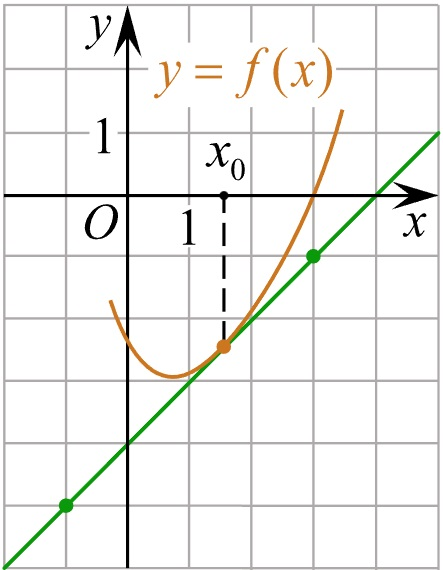
\includegraphics[align=t, width=\linewidth]{\picpath/maksutovM8L4-3}
		\end{minipage}
		\item
		\begin{minipage}[t]{\bodywidth}
			На рисунке изображены график функции \(y=f(x)\) и касательная к этому графику, проведённая в точке \(x_0\). Уравнение касательной показано на рисунке. Найдите значение производной функции \(g(x)=-7f(x)+21x+\dfrac{ 1 }{ 441 }\) в точке \(x_0\).
		\end{minipage}
		\hspace{0.02\linewidth}
		\begin{minipage}[t]{\picwidth}
			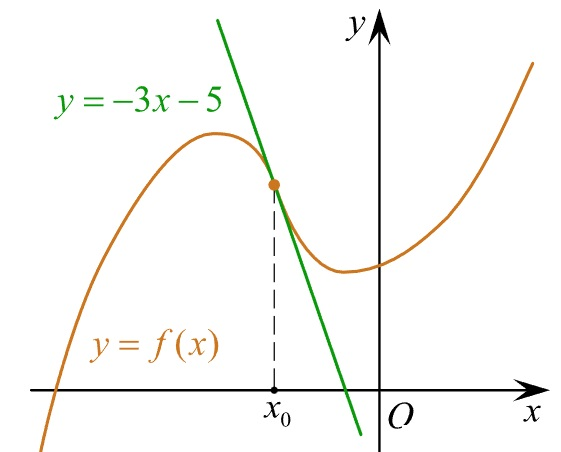
\includegraphics[align=t, width=\linewidth]{\picpath/G112M8C3-1}
		\end{minipage}
		%525702
			\item
		\begin{minipage}[t]{\bodywidth}
			На рисунке изображены график функции \(y=f(x)\) и касательная к этому графику, проведённая в точке \(x_0\). Уравнение касательной показано на рисунке. Найдите значение производной функции \(g(x)=f'(x)-f(x)+3\) в точке \(x_0\).
		\end{minipage}
		\hspace{0.02\linewidth}
		\begin{minipage}[t]{\picwidth}
			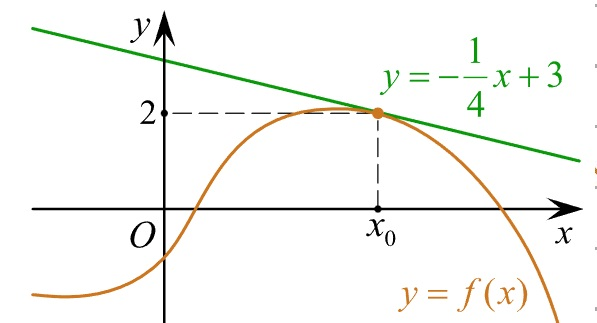
\includegraphics[align=t, width=\linewidth]{\picpath/G112M8C3-4}
		\end{minipage}
		%541816
		\item
		\begin{minipage}[t]{\bodywidth}
			На рисунке изображены график функции \(y=f(x)\) и касательная к нему в точке с абсциссой \(x_0\). Найдите значение производной функции \(f(x)\)в точке \(x_0\).
		\end{minipage}
		\hspace{0.02\linewidth}
		\begin{minipage}[t]{\picwidth}
			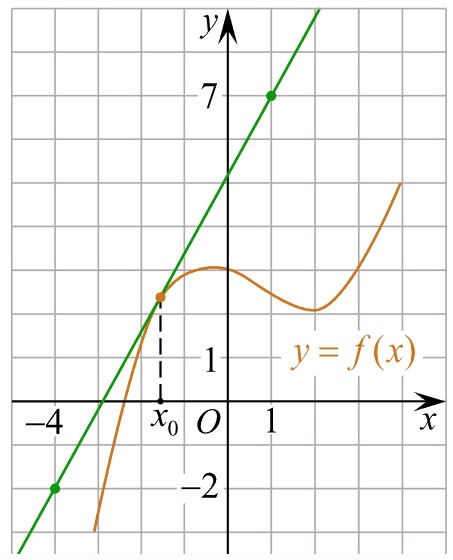
\includegraphics[align=t, width=\linewidth]{\picpath/maksutovM8L4-1}
		\end{minipage}
		%9063
	\end{listofex}
\end{class}
%END_FOLD